\documentclass[times, utf8, zavrsni]{fer}
\usepackage{booktabs,appendix,listings,hyperref,graphicx,float}
\graphicspath{ {img/} }

\begin{document}

\thesisnumber{4942}

\title{Sustav za sigurno i učinkovito udaljeno izvođenje studentskih programskih vježbi}

\author{Petar Šegina}

\maketitle

% Ispis stranice s napomenom o umetanju izvornika rada. Uklonite naredbu \izvornik ako želite izbaciti tu stranicu.
\izvornik

% Dodavanje zahvale ili prazne stranice. Ako ne želite dodati zahvalu, naredbu ostavite radi prazne stranice.
\zahvala{}

\tableofcontents

\chapter{Uvod}

U redovnoj nastavi Fakulteta elektrotehnike i računarstva studenti se nerijetko susreću sa zadaćama čija je rješenja potrebno ostvariti pisanjem programa u odgovarajućim programskim jezicima. Ručno vrednovanje takvih rješenja bio bi dug i težak posao te se zato u sklopu određenih kolegija za vrednovanje rješenja koriste automatizirani sustavi.

Princip rada takvih sustava je jednostavan - svaki student svoje rješenje piše po specifikaciji koja zahtijeva da program sa standardnog ulaza učita ulazne podatke te na standardni izlaz ispiše rješenje izvođenja u nekom strukturiranom zapisu. Sve što sustav za evaluaciju mora poznavati da bi dobro odradio svoj posao je jedan ili više parova ulaza i očekivanog izlaza. Algoritam sustava za izvršavanje može se zatim svesti na sljedeće:

\begin{enumerate}
\item Prevedi izvorni kod u izvršni oblik
\item Pokreni program
\item Na standardni ulaz programa proslijedi ulazne podatke
\item Čekaj kraj programa
\item Sakupi izlaz programa
\item Usporedi dobiveni izlaz s očekivanim i javi rezultat
\end{enumerate}

Iako se taj posao na prvi pogled čini jednostavnim, iza navedenih koraka skriva se mnogo izazova od kojih su neki:

\begin{enumerate}
\item Kako prevesti kod u izvršni oblik?
	\begin{itemize}
	\item Koje programske jezike i okruženja podržati?
	\item Koje inačice programskih jezika i okruženja podržati?
	\item Kako ostvariti podršku za više sličnih izvršnih okolina na jednom sustavu?
	\item Što ako se program ne uspije uspješno prevesti?
	\end{itemize}
\item Kako sigurno i uspješno izvršiti program?
	\begin{itemize}
	\item Što ako program sadrži grešku i neće nikada završiti?
	\item Što ako je program maliciozan i pokuša naškoditi izvršnoj okolini?
	\end{itemize}
\item Kako vrednovati dodatna svojstva rješenja?
	\begin{itemize}
	\item Možemo li prihvatiti samo rješenja koja izvršavanje završe u određenom vremenu?
	\item Možemo li prihvatiti samo rješenja koja koriste određenu količinu memorije?
	\end{itemize}
\end{enumerate}

Uz sve to, sustav za vrednovanje također mora biti efikasan. Primjera radi, ako kolegij upiše 600 studenata, od čega ih 500 preda rješenje laboratorijske vježbe te ako se vrednovanje te vježbe sastoji od 20 testnih primjera koji se u prosjeku svaki izvršava pet sekundi, za evaluaciju laboratorijske vježbe bit će potrebno 500*20*5 = 50.000 sekundi ili otprilike 14 sati, ako ispitivanje provodimo jedan po jedan primjer.

Idealan sustav za vrednovanje rješenja trebao bi biti brz, efikasan, siguran i lak za korištenje. U nastavku ćemo prvo promotriti par postojećih rješenja, a zatim opisati implementaciju vlastitog sustava temeljenog na tehnologiji {\textit{Docker}}. Ostvareni sustav temeljen je na svojstvu razmjernog rasta kako bi se izvršavanje moglo rasporediti na neograničen broj nezavisnih sustava. Također nudi i fleksibilnost po pitanju izvršnih okolina koje su podržane te je jednostavan za postaviti i koristiti.

% TODO neki hook zašto je ostvareni sustav kul

\chapter{Postojeći sustavi}

Osvrnimo se prvo na nekoliko postojećih sustava za izvršavanje i evaluaciju programskih rješenja. Sustave navodimo dijelom jer su poslužili kao inspiracija u razvoju našeg rješenja zbog svojih inovativnih pristupa, a dijelom jer su valjane alternative koje treba razmotriti i uzeti u obzir prilikom odabira sustava za evaluaciju.

\section{SPRUT}

SPRUT{\footnote{\url{https://balrog.zemris.fer.hr/}}} je sustav za vrednovanje studentskih vježbi koji se koristi automatsko vrednovanje studentskih laboratorijskih vježbi na Fakultetu elektrotehnike i računarstva u sklopu kolegija poput {\textit{Uvod u teoriju računarstva (86537)}}{\footnote{\url{https://www.fer.unizg.hr/predmet/utrz}}} te {\textit{Prevođenje programskih jezika (86504)}}{\footnote{\url{https://www.fer.unizg.hr/predmet/ppj_a}}}.

Iako SPRUT trenutno zadovoljava potrebe na trenutnim kolegijima, mana mu je serijski način izvođenja i nemogućnost razmjernog rasta, zbog čega vrednovanje studentskih vježbi traje dugo te je jedina mogućnost za optimizaciju vertikalni rast, tj. kupovina bržeg hardvera.

\section{CodeAssign}

CodeAssign{\footnote{\url{https://codeassign.com/}}} je sustav nastao kao studentski projekt u sklopu kolegija {\textit{Oblikovanje programske potpore (34269)}}{\footnote{\url{https://www.fer.unizg.hr/predmet/opp}}}. CodeAssign je zamišljen kao mjesto gdje studenti, profesori i svi ostali zainteresirani mogu dijeliti programske zadatke i vježbe čija se rješenja automatizirano vrednuju.

Ono što CodeAssign razlikuje od ostalih rješenja je to što se sve izvršavanje koda događa na klijentu, dok poslužitelj samo potvrđuje valjanost dobivenog izlaza. Prednost takvog pristupa je znatno jednostavnija arhitektura poslužitelja, koji samo mora uspoređivati dobiveni izlaz s očekivanim te puno veća fleksibilnost na klijentu - korisnik sam odabire programsku okolinu u kojoj će raditi te se sam mora pobrinuti da ista radi.

Kako CodeAssign ne dolazi u dodir s izvornim kodom rješenja niti izvršava sam program, nije prikladan za vrednovanje laboratorijskih vježbi jer ne može potvrditi valjanost programskog rješenja. S druge strane, zbog lakoće korištenja i održavanja te fleksibilnosti u odabiru programske okoline smatramo ga dobrim odabirom za jednostavnije vježbe čija je svrha utvrđivanje i lakše praćenje gradiva.

CodeAssign je većinskim dijelom otvorenog koda{\footnote{\url{https://github.com/codeassign}}} te sama implementacija se može koristiti i u obrazovne svrhe.

\section{Judge0}

Judge0{\footnote{\url{http://judge0.com/}}} je javno dostupan sustav otvorenog koda{\footnote{\url{https://github.com/judge0}}} koji nudi uslugu sigurnog izvršavanja potencijalno malicioznog izvornog koda.

Prednost Judge0 je u tome što sustav nudi jednostavno programsko sučelje kojim se mogu zakazati izvođenja programa, dok mu je mana to što nije namijenjen razmjernom rastu te također obrađuje zadatke serijski. 

\section{Evaluator}

Evaluator{\footnote{\url{https://evaluator.mioc.hr/}}} je sustav koji se koristi u redovnoj nastavi zagrebačke XV. gimnazije te u sklopu vještine {\textit{Natjecateljsko programiranje (65973)}}{\footnote{\url{https://www.fer.unizg.hr/predmet/natpro}}} na Fakultetu elektrotehnike i računarstva.

Kako se redovno koristi u nastavi, Evaluator je postao robustan i stabilan sustav s podrškom za različitim izvršnim okolinama te naprednim mogućnostima poput razmjernog rasta dodavanjem novih radilica te preciznog definiranja ograničenja na vrijeme izvođenja.

Mana Evaluatora je u tome što se radi o zatvorenom sustavu kojeg ne možemo jednostavno preuzeti i prilagoditi svojim potrebama.

\chapter{Sustav za sigurno i učinkovito udaljeno izvođenje studentskih programskih vježbi}

\section{Korištene tehnologije}

Prije samog opisa ostvarenja sustava dajemo kratak pregled korištenih tehnologija kako bi olakšali praćenje i razumijevanje samog postupka implementacije.

\subsection{Docker}

Veoma pojednostavljeno, Docker{\footnote{\url{https://www.docker.com/}}} je tehnologija koja nam omogućava da u jednu crnu kutiju, osim samih izvršnih datoteka, također upakiramo i cijelu okolinu (\textit{userspace} operativnog sustava) u kojoj se naš program izvršava. Posljedica toga je da, ako želimo pokrenuti program X na svome računalu ili poslužitelju (gdje X može biti jednostavna \textit{hello-world} aplikacija ili složeni mrežni sustav), ne moramo brinuti o tome u kojem je jeziku taj program pisan te koje sve ovisnosti i preduvjete moramo zadovoljiti prije pokretanja. Docker nam omogućava da svaki program apstrahiramo na crnu kutiju s jasno definiranim ulazima i izlazima.

Docker sve više raste u popularnosti te je za očekivati da će postati \textit{de facto} standard za postavljanje i pokretanje programa i web usluga. Unutar ovog projekta ga koristimo iz istog razloga - svi mikroservisi nude svoje Docker slike kako bi se cijeli sustav jednostavnije mogao postaviti i pokrenuti. No, također ga koristimo i za pojednostavljenu izgradnju i izvršavanje studentskih rješenja, o čemu će više riječi biti kasnije.

\subsection{Spring}

Naš sustav ostvarili smo u obliku više nezavisnih mikroservisa kako bi osigurali mogućnost razmjernog rasta. Mikroservise smo ostvarili u programskom okviru Spring{\footnote{\url{https://spring.io/}}} jer je autor imao prijašnjeg iskustva s istim, a on nam je omogućio brz razvoj mikroservisa povezanih protokolom HTTP te brzu i jednostavnu implementaciju komunikacije s bazom podataka.

\subsection{Kotlin}

Kotlin{\footnote{\url{https://kotlinlang.org/}}} je programski jezik koji se nedavno pojavio te je uzeo velikog maha u zajednici osoba koje razvijaju programska rješenja za platformu Android. Radi se o modernom programskom jeziku koji se (među ostalim) prevodi u Java bytekod te nudi potpunu interoperabilnost s postojećim JVM tehnologijama.

Od prednosti nad programskim jezikom Java istaknuti ćemo sigurniji i bolji sustav tipova, jednostavniju i izražajniju sintaksu te bolju podršku za određene konstrukte funkcijskog programiranja.

Kotlin smo koristili za izradu svih mikroservisa i pomoćnih biblioteka. 

\subsection{H2}

Kako u nekom trenutku moramo spremiti rezultate vrednovanja, odlučili smo ih spremiti u relacijsku bazu podataka. Za tu komponentu smo odabrali bazu H2{\footnote{\url{http://www.h2database.com/html/main.html}}} jer korišteni programski okvir Spring Data ima odličnu podršku za istu. Također, H2 može svoje podatke spremati u običnu datoteku na datotečnom sustavu što nam pojednostavljuje proces postavljanja i održavanja baze podataka.

\section{Idejno ostvarenje}

Prije opisivanja ideje ostvarenja, podsjetimo se što očekujemo od sustava kojeg želimo napraviti, ali i koristiti:

\begin{enumerate}
\item Sigurnost
\item Mogućnost razmjernog rasta (\textit{skalabilnost})
\item Efikasnost
\item Jednostavnost korištenja
\end{enumerate}

Glavni alat na kojem ćemo bazirati svoje rješenje jesu izvršne Docker slike. Naime, Docker nam omogućava da bilo koji program upakiramo, zajedno s njegovom izvršnom okolinom, u crnu kutiju koju zatim možemo izvršiti poput izvršne datoteke. Sve što nam je pritom potrebno je Docker okolina te ne ovisimo o implementacijskim detaljima programa kojeg izvršavamo. Izvršne Docker slike možemo pojednostavljeno smatrati kako statično povezivanje na steroidima - u kutiji uz program dolazi i cijeli \textit{userspace} operativnog sustava nad kojim će se program izvršiti.

Iduća veoma korisna činjenica je ta da u samu Docker sliku možemo \textit{upeći} ulazne podatke koje će program primiti. Tako ćemo dobiti izvršnu Docker sliku koja će za deterministički program uvijek davati jednak izlaz, neovisno o tome gdje je pokrenuta, a možemo ju pokrenuti bilo gdje, gdje imamo pristup Dockeru.

Prije nego što možemo rješenje izvršiti, moramo prilikom generiranja Docker slike ponuditi ili izvršnu okolinu za interpretirane jezike ili prevedene datoteke za jezike koji se prevode. Ovaj korak je individualan za svaki jezik, a detalje ćemo ponuditi nešto kasnije.

Zadnja stvar koja će nas zanimati je kako je tekao proces prevođenja i izvršavanja samog programa te koji je njegov konačni ispis. Prilikom izvršavanja izvršne Docker slike, standardni izlaz programa bit će vidljiv na ekranu. No, kako bi mogli automatizirati evaluaciju te obrađivati izlaz, morat ćemo ga proslijediti na udaljenu lokaciju. To možemo ostvariti tako da prilikom izvršavanja sam program omotamo u drugi program koji će uhvatiti njegov izlaz i proslijediti ga na odgovarajuću lokaciju. No, kako želimo zadržati fleksibilnost, cilj nam je udaljenu lokaciju na koju će se slati informacije o izvršavanju na neki način parametrizirati. Izvršne Docker slike nam i to omogućuju te možemo prilikom izvršavanja slike također predati i dodatne argumente, što ćemo iskoristiti za parametriziranje udaljene lokacije na koju će se slati informacije o izvršavanju.

Uzimanjem svega navedenog u obzir, koristeći izvršne Docker slike možemo dobiti \textit{nešto} što će svojim pokretanjem rezultate izvršavanja programa poslati na neku udaljenu lokaciju. Idealni poziv takve slike bio bi:

\begin{lstlisting}
./nesto https://mojaudaljenalokacija
\end{lstlisting}

što bi unutar sebe pokrenulo program koji vrednujemo i informacije o toku izvršavanja poslalo na udaljeno web sjedište {\textit{mojaudaljenalokacija}}. U stvarnosti će taj poziv izgledati ovako:

\begin{lstlisting}[language=Bash]
docker run --rm -it \
	sandworm/images/test_image/compiled/hello_petar \
	https://sandworm-logger/neki-tag
\end{lstlisting}

što će pokrenuti Docker sliku kreiranu za navedeni program i proslijediti pokretaču unutar nje lokaciju na koju treba poslati informacije o izvršavanju.

Rezultat ovog pristupa je taj da nam nije bitno gdje se izvršavanje događa te kamo se usmjerava rezultat izvršavanja. To nam omogućava da veoma lako ostvarimo svojstvo razmjernog rasta - radilica koje će izvršavati programe možemo imati proizvoljno mnogo, a isto to možemo napraviti i sa servisima koji će skupljati informacije o izvršavanju. Ono što će nam još trebati je servis ili alat koji će se brinuti o zakazivanju izvršavanja - na kojoj će se radilici izvesti koja slika te kamo će ona proslijediti rezultat izvođenja.

Konačno, cijeli proces vrednovanja možemo opisati sljedećim koracima:

\begin{enumerate}
\item Za svaki par (program, ulazna definicija) generirati izvršnu Docker sliku s potpuno fiksiranim kontekstom izvršavanja
\item Pokrenuti sliku na nekoj radilici s Docker podrškom - samo pokretanje će slati informacije o izvršavanju na udaljenu lokaciju
\item Preuzeti rezultate izvršavanja s nekog servisa za praćenje izvršavanja
\end{enumerate}

Dodatno, ako prilikom pokretanja ne navedemo udaljenu lokaciju na koju će se slati informacije o izvršavanju, možemo program pokrenuti bez funkcionalnosti skupljanja podataka. Time smo dobili crnu kutiju koja, jednom kad se pokrene, izvrši korisnički program s jednim točno definiranim skupom podataka. Korisna posljedica je ta da smo dobili jednostavan način reprodukcije rezultata pokretanja koji ne ovisi o platformi na kojoj se program pokreće. Tako, ako student nije zadovoljan rezultatom vrednovanja svog programa, može pokrenuti generiranu sliku lokalno i uvjeriti se u ispis svog programa.

Konkretan sustav ostvaren je kao skup nezavisnih alata i mikroservisa koji obavljaju navedene zadaće, a detaljnije ćemo ih opisati u nastavku.

\section{Logička arhitektura}

Kao što smo već naveli, sam sustav ostvaren je kao skup nezavisnih alata i mikroservisa. Logička arhitektura koja prikazuje način na koji su manje jedinice spojene u funkcionalnu cjelinu prikazan je u nastavku.

\begin{figure}[H]
	\centering
	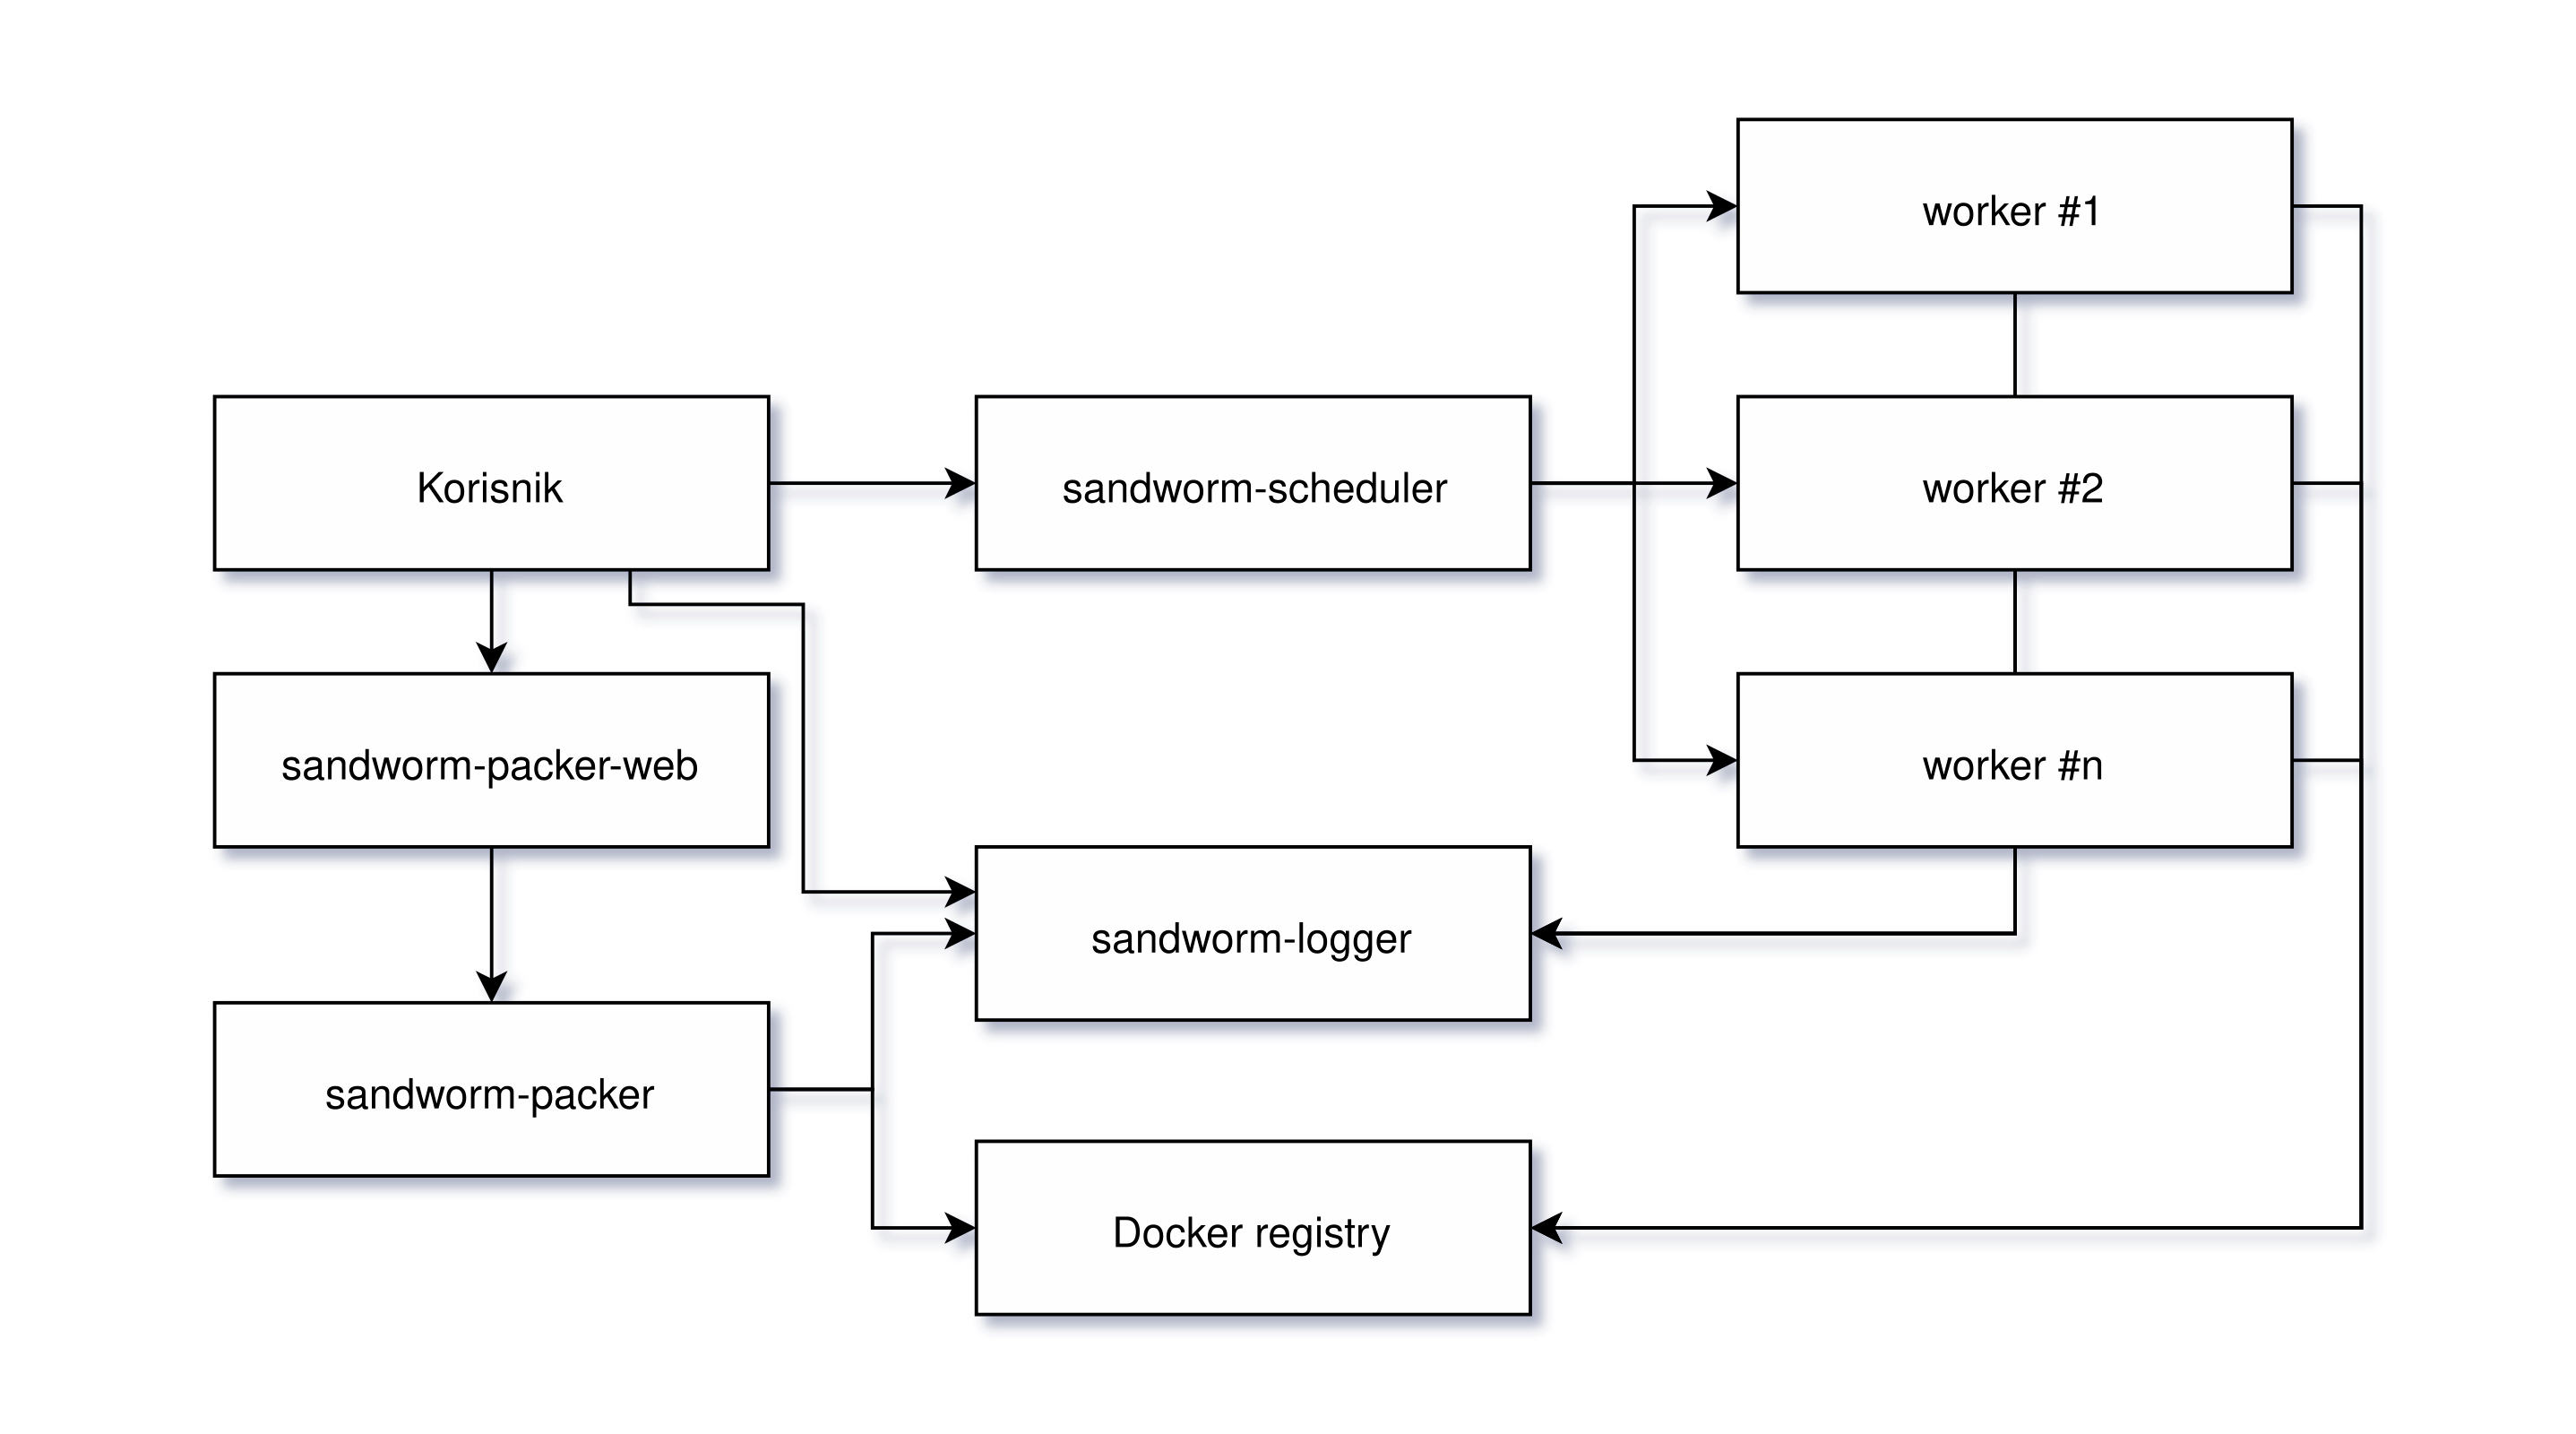
\includegraphics[width=\textwidth]{sandworm-schema.png}
	\caption{Prikaz logičke arhitekture sustava}
\end{figure}

Alati s kojima korisnik dolazi u susret su usluga za pakiranje ulaznih podataka i izvršnog koda u izvršne Docker slike, {\textit{sandworm-packer-web}}, usluga za zakazivanje i izvršavanje kreiranih slika, {\textit{sandworm-scheduler}} te usluga za prikupljanje i skladištenje rezultata, {\textit{sandworm-logger}}.

\hfill
\break

Zamišljena interakcija korisnika (fizičkog ili drugog programa) je sljedeća:

\begin{enumerate}
\item Na uslugu za pakiranje korisnik šalje ulaznu definiciju programa kojeg vrednuje - naziv izvršne okoline, izvorni kod, skup ulaznih datoteka, lokaciju zapisivanja rezultata postupka pakiranja te proizvoljan naziv pod kojim će biti spremljene informacije o pakiranju te na temelju kojeg će biti generirani nazivi Docker slika. Jednom kada poziv završi, u dijeljenom registru Docker slika ({\textit{Docker registry}}) nalazit će se slike za svaki ulazni podatak te jedna slika bez ulaznih podataka, ali s prevedenim programom.
\item Na uslugu za zakazivanje izvođenja korisnik za svaku generiranu sliku šalje novi zahtjev u kojem definira putanju do dijeljenog registra, naziv slike te putanju do usluge za prikupljanje i skladištenje rezultata. Usluga će zatim zakazati izvršavanje na jednoj od radilica ({\textit{worker \#n}}) te informaciju o tome poslati na uslugu za prikupljanje i skladištenje rezultata. Jednom kada izvršavanje završi, u toj istoj usluzi će se nalaziti i informacija o tijeku izvođenja te prikupljeni standardni izlaz programa.
\item Korisnik na temelju naziva kojeg je zadao u prvom koraku s usluge za prikupljanje i skladištenje rezultata povlači informacije o tijeku pakiranja, prevođenja i izvršavanja.
\end{enumerate}

Usluga za pakiranje rješenja i ulaznih definicija ({\textit{sandworm-packer-web}}) ostvarena je kao jednostavan omotač oko biblioteke za pakiranje rješenja i ulaznih definicija ({\textit{sandworm-packer}}) koja je ostvarena kao zaseban alat kojeg možemo koristiti iz komandne linije te ju zato posebno ističemo na shemi logičke arhitekture.


\section{Ostvarenje}

Na idućih nekoliko strana opisat ćemo konkretno ostvarenje sustava. Projekt je, sukladno logičkoj arhitekturi, podijeljen na odgovarajuće podprojekte. Oni su:

\begin{enumerate}
\item {\textit{sandworm-images}} - temeljne Docker slike potrebne za izgradnju izvršnih Docker slika s podrškom za razne izvršne okoline
\item {\textit{sandworm-packer}} - biblioteka i komandnolinijski alat za pakiranje ulaznih definicija u izvršne Docker slike
\item {\textit{sandworm-packer-web}} - web usluga za pristup funkcionalnosti alata za pakiranje
\item {\textit{sandworm-scheduler}} - usluga za zakazivanje izvođenja i upravljanje radilicama
\item {\textit{sandworm-whitepaper}} - izvorne datoteke ovog rada
\end{enumerate}


\subsection{Temeljne slike s izvršnim okolinama za pojedine jezike}

Kako bi sustav mogao podržati različite okoline izvršavanja bilo je potrebno napraviti nekoliko temeljnih Docker slika nad kojima će se graditi konačne izvršne slike. Točnije, za svaku željenu okolinu (npr. C, C++, JavaScript) potrebno je napraviti zasebnu sliku. Iako smo mogli napraviti jednu sliku koja bi sadržavala sve okoline, ovaj smo pristup odabrali zbog veće fleksibilnosti. Pojedine slike su veoma jednostavne i lakše za održavati u odnosu na jednu veliku sliku.

Svaka slika u svojem direktoriju sadrži skriptu {\textit{build.sh}} kojom se slika može izgraditi i koja označava sliku odgovarajućom oznakom. U vršnom direktoriju podprojekta nalazi se skripta {\textit{build.sh}} koja gradi sve pojedinačne slike.

\subsubsection{Temeljna slika}

Temeljna slika ({\textit{base}}) sadrži skripte koje nude osnovne funkcionalnosti sustava zajedničke svim okolinama. One su:

\begin{enumerate}
\item {\textit{compile.sh}} - skripta koja izvodi prevađanje izvornog koda u strojni kod za okoline u kojima je to potrebno
\item {\textit{stream-collector.sh}} - skripta koja šalje proizvoljan ispis na uslugu za prikupljanje i skladištenje rezultata
\item {\textit{entrypoint.sh}} - skripta koja omata skriptu {\textit{runner.sh}} i pomoću {\textit{stream-collector.sh}} šalje njen izlaz i izlaz za greške na uslugu za prikupljanje i skladištenje rezultata, definiranu kao prvi argument skripte
\end{enumerate}

Iako {\textit{entrypoint.sh}} poziva skriptu {\textit{runner.sh}}, ona nije dio temeljne slike. Naprotiv, nju će ponuditi slike specifične za svaku okolinu, jer ona određuje kako se program izvršava i kako mu se predaju ulazni podaci.

Sama definicija temeljne slike dostupna u datoteci {\textit{Dockerfile}} veoma je jednostavna:

\begin{lstlisting}
FROM ubuntu:16.04

RUN apt-get update \
    && apt-get install -y --no-install-recommends curl \
    && apt-get clean \
    && rm -rf /var/lib/apt/lists/* /tmp/* /var/tmp/*

COPY compile.sh .
COPY entrypoint.sh .
COPY stream-collector.sh .

ENTRYPOINT ["/bin/bash", "./entrypoint.sh"]
\end{lstlisting}

Slika prvo definira izvornu sliku za koju smo odabrali Ubuntu 16.04. Zatim u sebe kopira pomoćne skripte te na kraju definira skriptu {\textit{entrypoint.sh}} kao {\textit{entrypoint}} Docker slike, tj. skriptu koja će biti pokrenuta ako Docker sliku pokrenemo kao izvršni program.

Temeljna slika je sama po sebi beskorisna jer joj nedostaje ključna skripta {\textit{runner.sh}}. Ako pokušamo izgraditi i pokrenuti temeljnu skriptu, dobit ćemo grešku zbog skripte koja nedostaje. Da bi dobili izvršno okruženje koje radi moramo još definirati i instalaciju okruženja te način pozivanja programa.

\subsubsection{C i C++}

Idući korak je definiranje slika s izvršnim okruženjima pa ćemo početi sa okruženjem za programske jezike C i C++. Pogledajmo prvo definiciju slike u datoteci {\textit{Dockerfile}}:

\begin{lstlisting}
FROM sandworm/base/base

RUN apt-get update \
    && apt-get install -y --no-install-recommends build-essential \
    && apt-get clean \
    && rm -rf /var/lib/apt/lists/* /tmp/* /var/tmp/*

COPY runner.sh .
\end{lstlisting}

Za podršku za programske jezike C i C++ dovoljno je nad temeljnom slikom instalirati paket {\textit{build-essential}} (koji sadrži alate gcc i g++ potrebne za prevođenje koda) te ponuditi skriptu za pokretanje programa, {\textit{runner.sh}}. Pogledajmo i njenu definiciju:

\begin{lstlisting}
#!/usr/bin/env bash

./a.out
\end{lstlisting}

Sve što je potrebno za pokrenuti preveden program je pokrenuti izvršnu datoteku koja je generirana procesom prevođenja u skripti {\textit{compile.sh}} u temeljnoj slici, dok će se za preusmjeravanje ulaznih podataka te hvatanja izlaznih podataka pobrinuti omatajuća skripta {\textit{entrypoint.sh}}.

Zbog arhitekturalnih ograničenja je postupak prevođenja potrebno definirati u temeljnoj slici. 

Dodavanje podrške za nove okoline, kao što je vidljivo iz priloženog, vrlo je jednostavno.

\subsubsection{JavaScript}

Za razliku od jezika C i C++, programski jezik JavaScript je interpretirani jezik. No, to ne utječe pretjerano na količinu posla potrebnu za dodavanje podrške i za tu okolinu. Datoteka {\textit{Dockerfile}} prati sličnu strukturu kao i ona za jezike C i C++:

\begin{lstlisting}
FROM sandworm/base/base

RUN apt-get update \
    && apt-get install -y --no-install-recommends nodejs \
    && apt-get clean \
    && rm -rf /var/lib/apt/lists/* /tmp/* /var/tmp/*

COPY runner.sh .
\end{lstlisting}

Ovdje smo umjesto paketa {\textit{build-essential}} instalirali paket {\textit{nodejs}} koji nam nudi izvršno okruženje za programski jezik JavaScript.

Konačno, potrebno je i ponuditi skriptu za pokretanje izvršavanja, {\textit{runner.sh}}:

\begin{lstlisting}
#!/usr/bin/env bash

nodejs main.js
\end{lstlisting}

Slično kao i prije, potrebno je pozvati izvršnu okolinu nad datotekom koja sadrži izvorni kod. Ovdje smo se ograničili na to da rješenje mora imati datoteku naziva {\textit{main.js}} koja sadrži ulaznu točku u program. Ako bi ovo htjeli promijeniti, dovoljno je doraditi ovu sliku, ili na temelju nje napraviti drugu.

\subsubsection{Ostali jezici}

U gornje dvije slike prikazan je postupak dodavanja podrške za jedan prevedeni i jedan interpretirani jezik. Kako dodavanje podrške za druge jezike prati istu šablonu, nećemo ih više ovdje navoditi, dok sam projekt sadrži još slike za programske jezike Python 2 i Python 3.

\subsection{Praćenje i dijeljenje rezultata izvođenja}

\subsection{Alat za pakiranje rješenja i ulaznih definicija u izvršne Docker slike}

\subsection{Servis za prikupljanje i skladištenje rezultata}

\subsection{Servis za zakazivanje izvođenja i upravljanje radilicama}

\chapter{Vrednovanje}

\chapter{Daljnje dorade}

U nastavku iznosimo ideje za koje smatramo da bi bilo korisno razmotriti i implementirati kao proširenja postojećeg sustava.

\section{Vrednovanje ispisa programa}

Jedna od motivacija izgradnje ovog sustava bila je mogućnost zamjene SPRUT-a kao evaluacijskog mehanizma u kontekstu studentskih laboratorijskih vježbi.

Sustav koji smo napravili trenutno podržava samo izvršavanje programa, ali ne i evaluaciju. Točnije, s trenutnim ostvarenjem ne možemo automatizirano vrednovati rezultat izvođenja programskog rješenja.

Uzevši u obzir trenutnu arhitekturu sustava, vrednovanje ispisa moguće je ostvariti povlačenjem ispisa programa sa servisa za prikupljanje i skladištenje rezultata, filtriranje istih po oznaci stdout te uspoređivanje dobivenog s očekivanim izlazom. Sam ispis možemo dohvatiti na temelju oznake koju dobijemo prilikom zakazivanja izvršavanja programa.

Dodatno, osim standardnog izlaza, ništa nas ne sprječava da program vrednujemo i po drugim zapisima - recimo, na temelju zapisa možemo odrediti i je li bilo grešaka prilikom prevođenja te vrijeme koje je programu bilo potrebno da bi se izvršio.

Ukratko, trenutni sustav bilježi mnogo informacija na temelju kojih se može vrednovati ponašanje programa. Za izvedbu vrednovanja dovoljno je zakazati izvršavanje programa i zatim kasnije preuzeti informacije dostupne u servisu za prikupljanje i skladištenje rezultata.

\section{Unošenje izvršnih ograničenja}

Sustav trenutno nema podršku za definiranje izvršnih ograničenja (eng. {\textit{runtime constraints}}).

Izvršna ograničenja su nam korisna jer s njima možemo dodatno ograničiti izvođenje zadajući recimo najviše dozvoljeno vrijeme izvođenja, najviše dozvoljenu količinu iskorištene memorije ili najviše dozvoljen broj pokrenutih dretvi.

Izvršna ograničenja u postojećem sustavu mogu se ostvariti omatanjem skripte {\textit{runner.sh}} alatom {\textit{isolate}}\footnote{\url{https://github.com/ioi/isolate}}. {\textit{Isolate}} nam omogućava definiranje raznih izvršnih ograničenja nad bilo kojim programom pa tako i programima koje izvršavamo u sklopu našeg sustava.

Za izvršna ograničenja je bitno napomenuti da primjena istih ovisi o okolini u kojoj se program izvršava. Primjerice, naivna implementacija ograničenja ukupne memorije bi ograničila količinu memorije koju proces može zauzeti i ubila ga ako on istu prijeđe. No, tehnologije zasnovane na sakupljačima smeća često ne pokreću proces oslobađanja memorije dok sami ne zaključe da je to potrebno.

Primjerice, ako značajno ograničimo količinu memorije za proces koji izvršava kod pisan u programskom jeziku Java, a pritom ne obavijestimo virtualni stroj o ograničenjima (za JVM to možemo napraviti zastavicom {\textit{Xmx}}) isti nikad neće pokrenuti proces sakupljanja smeća te će program brzo nasilno završiti, iako je pisani program ispravan te ne bi zauzeo previše memorije ako bi se proces sakupljanja smeća na vrijeme pokrenuo.

Uz samu podršku za zadavanje izvršnih ograničenja korisno bi bilo dodati i mogućnost definiranja istih kao dio ulazne definicije programa. Primjerice, jedna datoteka {\textit{constraints.yml}} pisana u formatu YAML\footnote{\url{https://en.wikipedia.org/wiki/YAML}} mogla bi sadržavati lako čitljivu definiciju svih ograničenja.Tu datoteku bi zatim upekli u sliku te pomoću nje prilikom pokretanja konstruirali parametre za poziv alata {\textit{isolate}}. Dodatno, na temelju nje bi morali izgraditi i podršku za ograničenja za pojedine tehnologije izvršavanja u njihovim odgovarajućim slikama kako bi izbjegli probleme poput onog sa sakupljanjem smeća navedenog prije.


\section{Korištenje Infrastruktura-kao-Usluga sustava za automatsko provizioniranje radilica}

Sustav koji smo opisali trenutno se oslanja na predefiniran set radilica zapisanih unutar servisa za zakazivanje izvođenja i upravljanje radilicama. Posljedica je da, neovisno o količini programa koje trebamo evaluirati u danom trenutku radilice uvijek moraju biti spremne i pokrenute.

Predviđeno opterećenje sustava u akademskim uvjetima je skokovito - postojat će dugi periodi kada se sustav neće koristiti te kratki periodi kada će biti potrebno vrednovati velik broj studentskih rješenja.

Kako će radilice biti potrebne samo kratko vrijeme, predlažemo da se sustav za upravljanje radilicama doradi tako da ih automatski provizionira kada je to potrebno te ugasi kada više nisu potrebne. Primjerice, ako imamo fizičke strojeve koje koristimo kao radilice, sustav za upravljanje može koristiti tehnologiju {\textit{Wake-on-LAN}}{\footnote{\url{https://en.wikipedia.org/wiki/Wake-on-LAN}} kako bi strojeve palio i gasio po potrebi i tako uštedio na troškovima energije.

		  No, kako je posljedica naše arhitekture ta da nam uistinu nije bitno na čemu izvršavamo programe dokle god to nešto ima podršku za Docker, možemo se također osloniti i na Infrastruktura-kao-Usluga (eng. {\textit{Infrastructure-as-a-Service}}{\footnote{{\url{https://en.wikipedia.org/wiki/Cloud_computing}}}} sustave za automatsko provizioniranje radilica kada nam trebaju te gašenje istih kada nam ne trebaju. Ovim pristupom možemo ostvariti višu paralelizaciju izvođenja te smanjiti troškove jer takve usluge nude naplaćivanje po satu, što odgovara našim potrebama.

Tako bi mogli imati samo jedan fizički stroj lokalno koji bi brinuo o zaprimanju zahtjeva, dok bi sav težak posao mogli odraditi na dinamički provizioniranim radilicama.

Odabir ponuđača IaaS usluga ovisi ponajprije o cijeni te potrebama hardvera koji se zakupuje. Ponuđače koje ćemo spomenuti su {\textit{DigitalOcean}}{\footnote{\url{https://www.digitalocean.com/}}}, {\textit{Amazon Web Services}}{\footnote{\url{https://aws.amazon.com/}}}, {\textit{Microsoft Azure}}{\footnote{\url{https://azure.microsoft.com/}}} te {\textit{Google Cloud Platform}}{\footnote{\url{https://cloud.google.com/}}}. DigitalOcean, primjerice, nudi provizioniranje sustava unutar 55 sekundi što je prihvatljivo vrijeme čekanja u odnosu na trajanje cijelog procesa vrednovanja.

Za ostvarenje ove ideje bilo bi potrebno prilagoditi sustav za zakazivanje izvođenja i upravljanje radilicama tako da, umjesto unaprijed definiranog niza radilica, koristeći programska sučelja odgovarajućeg ponuđača usluga kreira i uništava radilice po potrebi. Konkretno, za ponuđača usluga DigitalOcean možemo iskoristiti biblioteku {\textit{digitalocean-api-java}}{\footnote{\url{https://github.com/jeevatkm/digitalocean-api-java}}}.

Po pitanju cijene i paralelizacije koju ovim pristupom možemo ostvariti, DigitalOcean u trenutku pisanja u svojoj ponudi, među ostalim, nudi i virtualne strojeve sa 512MB RAM, 20GB prostora za podatke te jednom virtualnom jezgrom što bi trebalo biti dovoljno za izvođenje studentskih vježbi. Cijena korištenja je \$0.007 po satu{\footnote{\url{https://www.digitalocean.com/pricing/}}} ili ugrubo 5 lipa po satu. Tako za trošak od kune po satu možemo pokrenuti ugrubo dvadeset strojeva koji će paralelno izvršavati i vrednovati studentske programe, što je i više nego prihvatljivo za naše potrebe.


\chapter{Zaključak}
Zaključak.

\begin{appendices}

\chapter{Upute za postavljanje}

\section{Preuzimanje izvornog koda}

\section{Pokretanje okoline uz pomoć alata Docker}

\section{Pokretanje okoline uz pomoć alata Gradle}

\chapter{Upute za korištenje}

\section{Dodavanje podrške za nova izvršna okruženja}

\section{Priprema izvornih datoteka za izvođenje}

\section{Zakazivanje izvršavanja}

\section{Dohvat rezultata izvršavanja}

\end{appendices}

\bibliography{literatura}
\bibliographystyle{fer}

\begin{sazetak}
Sažetak na hrvatskom jeziku.

\kljucnerijeci{Ključne riječi, odvojene zarezima.}
\end{sazetak}

\engtitle{Secure and Scalable Remote Execution of Students' Programming Assignments}
\begin{abstract}
Abstract.

\keywords{Keywords.}
\end{abstract}

\end{document}
